% Created by tikzDevice version 0.11 on 2018-12-11 10:42:19
% !TEX encoding = UTF-8 Unicode
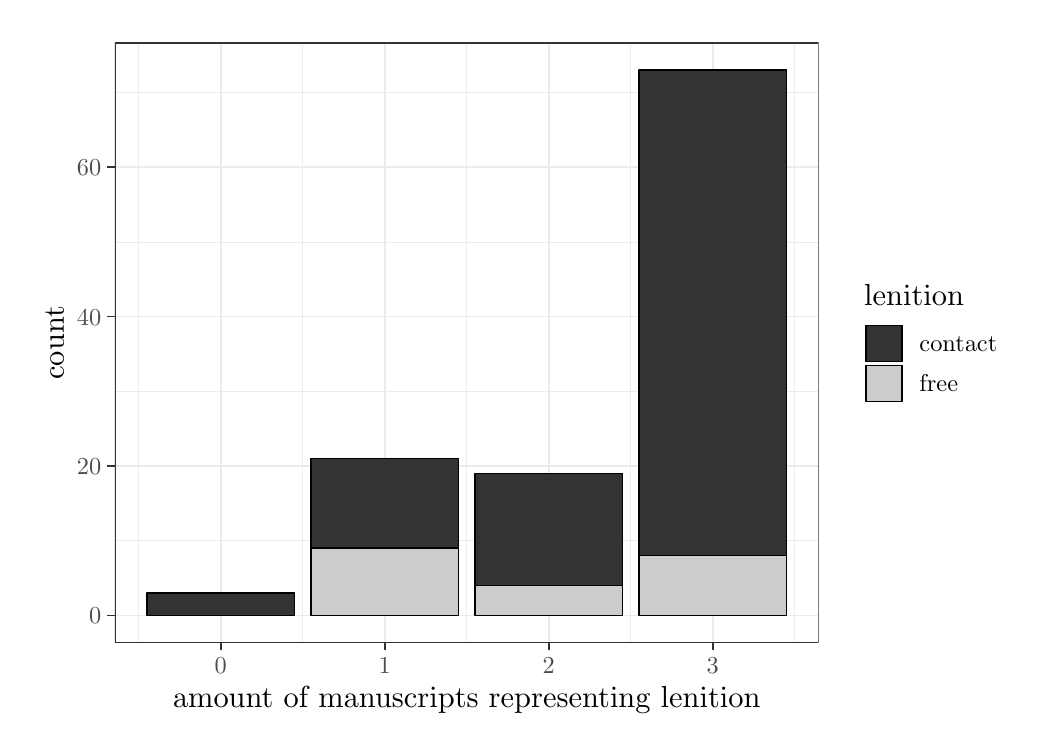
\begin{tikzpicture}[x=1pt,y=1pt]
\definecolor{fillColor}{RGB}{255,255,255}
\path[use as bounding box,fill=fillColor,fill opacity=0.00] (0,0) rectangle (361.35,252.94);
\begin{scope}
\path[clip] (  0.00,  0.00) rectangle (361.35,252.94);
\definecolor{drawColor}{RGB}{255,255,255}
\definecolor{fillColor}{RGB}{255,255,255}

\path[draw=drawColor,line width= 0.6pt,line join=round,line cap=round,fill=fillColor] (  0.00,  0.00) rectangle (361.35,252.94);
\end{scope}
\begin{scope}
\path[clip] ( 31.52, 30.72) rectangle (285.79,247.45);
\definecolor{fillColor}{RGB}{255,255,255}

\path[fill=fillColor] ( 31.52, 30.72) rectangle (285.79,247.45);
\definecolor{drawColor}{gray}{0.92}

\path[draw=drawColor,line width= 0.3pt,line join=round] ( 31.52, 67.56) --
	(285.79, 67.56);

\path[draw=drawColor,line width= 0.3pt,line join=round] ( 31.52,121.54) --
	(285.79,121.54);

\path[draw=drawColor,line width= 0.3pt,line join=round] ( 31.52,175.52) --
	(285.79,175.52);

\path[draw=drawColor,line width= 0.3pt,line join=round] ( 31.52,229.50) --
	(285.79,229.50);

\path[draw=drawColor,line width= 0.3pt,line join=round] ( 40.11, 30.72) --
	( 40.11,247.45);

\path[draw=drawColor,line width= 0.3pt,line join=round] ( 99.38, 30.72) --
	( 99.38,247.45);

\path[draw=drawColor,line width= 0.3pt,line join=round] (158.65, 30.72) --
	(158.65,247.45);

\path[draw=drawColor,line width= 0.3pt,line join=round] (217.93, 30.72) --
	(217.93,247.45);

\path[draw=drawColor,line width= 0.3pt,line join=round] (277.20, 30.72) --
	(277.20,247.45);

\path[draw=drawColor,line width= 0.6pt,line join=round] ( 31.52, 40.58) --
	(285.79, 40.58);

\path[draw=drawColor,line width= 0.6pt,line join=round] ( 31.52, 94.55) --
	(285.79, 94.55);

\path[draw=drawColor,line width= 0.6pt,line join=round] ( 31.52,148.53) --
	(285.79,148.53);

\path[draw=drawColor,line width= 0.6pt,line join=round] ( 31.52,202.51) --
	(285.79,202.51);

\path[draw=drawColor,line width= 0.6pt,line join=round] ( 69.75, 30.72) --
	( 69.75,247.45);

\path[draw=drawColor,line width= 0.6pt,line join=round] (129.02, 30.72) --
	(129.02,247.45);

\path[draw=drawColor,line width= 0.6pt,line join=round] (188.29, 30.72) --
	(188.29,247.45);

\path[draw=drawColor,line width= 0.6pt,line join=round] (247.56, 30.72) --
	(247.56,247.45);
\definecolor{drawColor}{RGB}{0,0,0}
\definecolor{fillColor}{gray}{0.20}

\path[draw=drawColor,line width= 0.6pt,line join=round,fill=fillColor] ( 43.08, 40.58) rectangle ( 96.42, 48.67);
\definecolor{fillColor}{gray}{0.80}

\path[draw=drawColor,line width= 0.6pt,line join=round,fill=fillColor] (102.35, 40.58) rectangle (155.69, 64.87);
\definecolor{fillColor}{gray}{0.20}

\path[draw=drawColor,line width= 0.6pt,line join=round,fill=fillColor] (102.35, 64.87) rectangle (155.69, 97.25);
\definecolor{fillColor}{gray}{0.80}

\path[draw=drawColor,line width= 0.6pt,line join=round,fill=fillColor] (161.62, 40.58) rectangle (214.96, 51.37);
\definecolor{fillColor}{gray}{0.20}

\path[draw=drawColor,line width= 0.6pt,line join=round,fill=fillColor] (161.62, 51.37) rectangle (214.96, 91.85);
\definecolor{fillColor}{gray}{0.80}

\path[draw=drawColor,line width= 0.6pt,line join=round,fill=fillColor] (220.89, 40.58) rectangle (274.23, 62.17);
\definecolor{fillColor}{gray}{0.20}

\path[draw=drawColor,line width= 0.6pt,line join=round,fill=fillColor] (220.89, 62.17) rectangle (274.23,237.59);
\definecolor{drawColor}{gray}{0.20}

\path[draw=drawColor,line width= 0.6pt,line join=round,line cap=round] ( 31.52, 30.72) rectangle (285.79,247.45);
\end{scope}
\begin{scope}
\path[clip] (  0.00,  0.00) rectangle (361.35,252.94);
\definecolor{drawColor}{gray}{0.30}

\node[text=drawColor,anchor=base east,inner sep=0pt, outer sep=0pt, scale=  0.88] at ( 26.57, 37.55) {0};

\node[text=drawColor,anchor=base east,inner sep=0pt, outer sep=0pt, scale=  0.88] at ( 26.57, 91.52) {20};

\node[text=drawColor,anchor=base east,inner sep=0pt, outer sep=0pt, scale=  0.88] at ( 26.57,145.50) {40};

\node[text=drawColor,anchor=base east,inner sep=0pt, outer sep=0pt, scale=  0.88] at ( 26.57,199.48) {60};
\end{scope}
\begin{scope}
\path[clip] (  0.00,  0.00) rectangle (361.35,252.94);
\definecolor{drawColor}{gray}{0.20}

\path[draw=drawColor,line width= 0.6pt,line join=round] ( 28.77, 40.58) --
	( 31.52, 40.58);

\path[draw=drawColor,line width= 0.6pt,line join=round] ( 28.77, 94.55) --
	( 31.52, 94.55);

\path[draw=drawColor,line width= 0.6pt,line join=round] ( 28.77,148.53) --
	( 31.52,148.53);

\path[draw=drawColor,line width= 0.6pt,line join=round] ( 28.77,202.51) --
	( 31.52,202.51);
\end{scope}
\begin{scope}
\path[clip] (  0.00,  0.00) rectangle (361.35,252.94);
\definecolor{drawColor}{gray}{0.20}

\path[draw=drawColor,line width= 0.6pt,line join=round] ( 69.75, 27.97) --
	( 69.75, 30.72);

\path[draw=drawColor,line width= 0.6pt,line join=round] (129.02, 27.97) --
	(129.02, 30.72);

\path[draw=drawColor,line width= 0.6pt,line join=round] (188.29, 27.97) --
	(188.29, 30.72);

\path[draw=drawColor,line width= 0.6pt,line join=round] (247.56, 27.97) --
	(247.56, 30.72);
\end{scope}
\begin{scope}
\path[clip] (  0.00,  0.00) rectangle (361.35,252.94);
\definecolor{drawColor}{gray}{0.30}

\node[text=drawColor,anchor=base,inner sep=0pt, outer sep=0pt, scale=  0.88] at ( 69.75, 19.71) {0};

\node[text=drawColor,anchor=base,inner sep=0pt, outer sep=0pt, scale=  0.88] at (129.02, 19.71) {1};

\node[text=drawColor,anchor=base,inner sep=0pt, outer sep=0pt, scale=  0.88] at (188.29, 19.71) {2};

\node[text=drawColor,anchor=base,inner sep=0pt, outer sep=0pt, scale=  0.88] at (247.56, 19.71) {3};
\end{scope}
\begin{scope}
\path[clip] (  0.00,  0.00) rectangle (361.35,252.94);
\definecolor{drawColor}{RGB}{0,0,0}

\node[text=drawColor,anchor=base,inner sep=0pt, outer sep=0pt, scale=  1.10] at (158.65,  7.44) {amount of manuscripts representing lenition};
\end{scope}
\begin{scope}
\path[clip] (  0.00,  0.00) rectangle (361.35,252.94);
\definecolor{drawColor}{RGB}{0,0,0}

\node[text=drawColor,rotate= 90.00,anchor=base,inner sep=0pt, outer sep=0pt, scale=  1.10] at ( 13.08,139.08) {count};
\end{scope}
\begin{scope}
\path[clip] (  0.00,  0.00) rectangle (361.35,252.94);
\definecolor{fillColor}{RGB}{255,255,255}

\path[fill=fillColor] (296.79,111.62) rectangle (355.85,166.55);
\end{scope}
\begin{scope}
\path[clip] (  0.00,  0.00) rectangle (361.35,252.94);
\definecolor{drawColor}{RGB}{0,0,0}

\node[text=drawColor,anchor=base west,inner sep=0pt, outer sep=0pt, scale=  1.10] at (302.29,152.50) {lenition};
\end{scope}
\begin{scope}
\path[clip] (  0.00,  0.00) rectangle (361.35,252.94);
\definecolor{fillColor}{RGB}{255,255,255}

\path[fill=fillColor] (302.29,131.57) rectangle (316.75,146.03);
\end{scope}
\begin{scope}
\path[clip] (  0.00,  0.00) rectangle (361.35,252.94);
\definecolor{drawColor}{RGB}{0,0,0}
\definecolor{fillColor}{gray}{0.20}

\path[draw=drawColor,line width= 0.6pt,line cap=round,fill=fillColor] (303.00,132.29) rectangle (316.03,145.32);
\end{scope}
\begin{scope}
\path[clip] (  0.00,  0.00) rectangle (361.35,252.94);
\definecolor{fillColor}{RGB}{255,255,255}

\path[fill=fillColor] (302.29,117.12) rectangle (316.75,131.57);
\end{scope}
\begin{scope}
\path[clip] (  0.00,  0.00) rectangle (361.35,252.94);
\definecolor{drawColor}{RGB}{0,0,0}
\definecolor{fillColor}{gray}{0.80}

\path[draw=drawColor,line width= 0.6pt,line cap=round,fill=fillColor] (303.00,117.83) rectangle (316.03,130.86);
\end{scope}
\begin{scope}
\path[clip] (  0.00,  0.00) rectangle (361.35,252.94);
\definecolor{drawColor}{RGB}{0,0,0}

\node[text=drawColor,anchor=base west,inner sep=0pt, outer sep=0pt, scale=  0.88] at (322.25,135.77) {contact};
\end{scope}
\begin{scope}
\path[clip] (  0.00,  0.00) rectangle (361.35,252.94);
\definecolor{drawColor}{RGB}{0,0,0}

\node[text=drawColor,anchor=base west,inner sep=0pt, outer sep=0pt, scale=  0.88] at (322.25,121.32) {free};
\end{scope}
\end{tikzpicture}
